\documentclass[10pt]{article}

%Math
\usepackage{amsmath}
\usepackage{amsfonts}
\usepackage{amssymb}
\usepackage{amsthm}
\usepackage{ulem}
%\usepackage{stmaryrd} %f\UTF{00FC}r Blitz!

%PageStyle
\usepackage[ngerman]{babel} % deutsche Silbentrennung
\usepackage[utf8]{inputenc} 
\usepackage{fancyhdr, graphicx}
\usepackage[scaled=0.92]{helvet}
\usepackage{enumitem}
\usepackage{parskip}
\usepackage[a4paper,top=2cm]{geometry}
\setlength{\textwidth}{17cm}
\setlength{\oddsidemargin}{-0.5cm}
\usepackage[scaled=0.92]{helvet}
\usepackage{lastpage} % for getting last page number
\renewcommand{\familydefault}{\sfdefault}


% Shortcommands
\newcommand{\Bold}[1]{\textbf{#1}} %Boldface
\newcommand{\Kursiv}[1]{\textit{#1}} %Italic
\newcommand{\T}[1]{\text{#1}} %Textmode
\newcommand{\Nicht}[1]{\T{\sout{$ #1 $}}} %Streicht Shit durch

%Arrows
\newcommand{\lra}{\leftrightarrow} 
\newcommand{\ra}{\rightarrow}
\newcommand{\la}{\leftarrow}
\newcommand{\lral}{\longleftrightarrow}
\newcommand{\ral}{\longrightarrow}
\newcommand{\lal}{\longleftarrow}
\newcommand{\Lra}{\Leftrightarrow}
\newcommand{\Ra}{\Rightarrow}
\newcommand{\La}{\Leftarrow}
\newcommand{\Lral}{\Longleftrightarrow}
\newcommand{\Ral}{\Longrightarrow}
\newcommand{\Lal}{\Longleftarrow}

% Code listenings
\usepackage{color}
\usepackage{xcolor}
\usepackage{listings}
\usepackage{caption}
\DeclareCaptionFont{white}{\color{white}}
\DeclareCaptionFormat{listing}{\colorbox{gray}{\parbox{\textwidth}{#1#2#3}}}
\captionsetup[lstlisting]{format=listing,labelfont=white,textfont=white}
\lstset{literate=%
    {Ö}{{\"O}}1
    {Ä}{{\"A}}1
    {Ü}{{\"U}}1
    {ß}{{\ss}}1
    {ü}{{\"u}}1
    {ä}{{\"a}}1
    {ö}{{\"o}}1
    {á}{{\'a}}1
    {í}{{\'i}}1
    {é}{{\'e}}1
    {ý}{{\'y}}1
    {ú}{{\'u}}1
    {ó}{{\'o}}1
    {é}{{\'{e}}}1
    {è}{{\`{e}}}1
    {È}{{\`{E}}}1
    {ê}{{\^{e}}}1
    {ë}{{\¨{e}}}1
    {É}{{\'{E}}}1
    {Ê}{{\^{E}}}1
    {û}{{\^{u}}}1
    {ù}{{\`{u}}}1
    {â}{{\^{a}}}1
    {à}{{\`{a}}}1
    {á}{{\'{a}}}1
    {ã}{{\~{a}}}1
    {Á}{{\'{A}}}1
    {Â}{{\^{A}}}1
    {Ã}{{\~{A}}}1
    {ç}{{\c{c}}}1
    {Ç}{{\c{C}}}1
    {õ}{{\~{o}}}1
    {ó}{{\'{o}}}1
    {ô}{{\^{o}}}1
    {Õ}{{\~{O}}}1
    {Ó}{{\'{O}}}1
    {Ô}{{\^{O}}}1
    {î}{{\^{i}}}1
    {Î}{{\^{I}}}1
    {í}{{\'{i}}}1
    {Í}{{\~{Í}}}1
    {ě}{{\v{e}}}1
    {š}{{\v{s}}}1
    {č}{{\v{c}}}1
    {ř}{{\v{r}}}1
    {ž}{{\v{z}}}1
    {ď}{{\v{d}}}1
    {ť}{{\v{t}}}1
    {ň}{{\v{n}}}1
    {ů}{{\r{u}}}1
    {Á}{{\'A}}1
    {Í}{{\'I}}1
    {É}{{\'E}}1
    {Ý}{{\'Y}}1
    {Ú}{{\'U}}1
    {Ó}{{\'O}}1
    {Ě}{{\v{E}}}1
    {Š}{{\v{S}}}1
    {Č}{{\v{C}}}1
    {Ř}{{\v{R}}}1
    {Ž}{{\v{Z}}}1
    {Ď}{{\v{D}}}1
    {Ť}{{\v{T}}}1
    {Ň}{{\v{N}}}1
    {Ů}{{\r{U}}}1
    {~}{{\textasciitilde}}1
}
\lstdefinestyle{JavaStyle}{
 language=java,
 basicstyle=\footnotesize\ttfamily, % Standardschrift
 numbers=left, % Ort der Zeilennummern
 numberstyle=\tiny, % Stil der Zeilennummern
 stepnumber=5, % Abstand zwischen den Zeilennummern
 numbersep=5pt, % Abstand der Nummern zum Text
 tabsize=2, % Groesse von Tabs
 extendedchars=true, %
 breaklines=true, % Zeilen werden Umgebrochen
 frame=b,
 %commentstyle=\itshape\color{LightLime}, Was isch das? O_o
 %keywordstyle=\bfseries\color{DarkPurple}, und das O_o
 basicstyle=\footnotesize\ttfamily,
 stringstyle=\color[RGB]{42,0,255}\ttfamily, % Farbe der String
 keywordstyle=\color[RGB]{127,0,85}\ttfamily, % Farbe der Keywords
 commentstyle=\color[RGB]{63,127,95}\ttfamily, % Farbe des Kommentars
 showspaces=false, % Leerzeichen anzeigen ?
 showtabs=false, % Tabs anzeigen ?
 xleftmargin=17pt,
 framexleftmargin=17pt,
 framexrightmargin=5pt,
 framexbottommargin=4pt,
 showstringspaces=false % Leerzeichen in Strings anzeigen ?
}

 
\fancypagestyle{firststyle}{ %Style of the first page
\fancyhf{}
\fancyheadoffset[L]{0.6cm}
\lhead{

\includegraphics[scale=0.8]{./fhnw_ht_e_10mm.jpg}}
\renewcommand{\headrulewidth}{0pt}
\lfoot{Institute of computer science,\linebreak www.fhnw.ch }
}

\fancypagestyle{documentstyle}{ %Style of the rest of the document
\fancyhf{}
\fancyheadoffset[L]{0.6cm}
\lhead{

\includegraphics[scale=0.8]{./fhnw_ht_e_10mm.jpg}}
\renewcommand{\headrulewidth}{0pt}
\lfoot{\thepage\ / \pageref{LastPage} }
}

\pagestyle{firststyle} %different look of first page
 
\title{ %Titel
Apsi-Lab 2
\vspace{0.2cm}
\Large Sichere Bearbeitung von HTML-Formularen}
\author{Jan Fässler \& Fabio Oesch}

\begin{document}
\maketitle
\thispagestyle{firststyle}
\pagestyle{firststyle}
\begin{abstract}
\begin{center}
Im Apsi-Lab 2 sollte eine Webseite mittels Servlets gebaut werden. Die Ziele waren Separation of privilege, Complete mediation, Fail-save defaults und Availability and reliability. Um sicher zu gehen, dass die Rechte auseiander gehalten werden, wurde ein Benutzer erstellt der nur auf die Datenbank schreiben und bearbeiten kann. Jeder Input wird mit einem Regex String verglichen damit diese keine Zeichen beinhalten können welche zu Angriffen benutzt werden können. Falls eine Attacke (SQL Injection oder XSS Attacke) versucht wird. Wird dies verhindert indem die Zeichen, die für die jeweilige Attacke benutzt werden, verändert werden. Die Applikation sollte ohne Probleme 50 Person parallel verarbeiten können. Dies ist jedoch abhängig vom Server.
\end{center}
\vspace{0.5cm}
\hrulefill
\end{abstract}

\pagestyle{documentstyle}
\tableofcontents
\pagebreak
\section{Einleitung}
\subsection{Ziel}
Die Bearbeitung von HTML-Formularen bildet das Rückgrat vieler Web-Applikationen. Mit
dieser Laborübung sollten Sie eine erste Schutzschicht (im Sinne von Saltzer und Schröder)
in Ihrer Web-Applikation sorgfältig planen und entwickeln. Sie sollen Ihre Aufmerksamkeit
auf die folgenden Grundprinzipien richten:
\begin{enumerate}
 \item  Separation of privilege: Halten Sie Rechte sorgfältig auseinander. Konkret will heissen,
dass die Programmschicht, welche die Eingaben des Benutzers sammelt, nicht auch für
den eigentlichen Login des registrierten Benutzers verwendet werden darf.
 \item  Complete mediation: Jeder Input/Output muss verifiziert werden. Sie sollten im Vor-
aus bestimmen, wie die erlaubte Information aussehen darf, und dann strikt die Kri-
terien für ihre Validierung formulieren.
 \item  Fail-safe defaults: Falls der Benutzer unbewusst (oder bewusst) falsche Informatio-
nen via HTML-Formular einschleusen will, sollte Ihre Applikation nur mit knappen
Hinweisen reagieren und vermeiden, dass der Benutzer die Applikation allzu lange
beansprucht (d.h. Sie sollten eine geeignete fail-safe Strategie entwerfen).
 \item  Availability and reliability: Ihre Applikation soll maximal 50 Benutzer in parallel (ohne
nennenswerte Einbussen in der Performanz) bedienen können. Überlegen Sie, welche
Implikationen diese Forderung für die Sicherheit Ihrer Applikation beinhaltet.
\end{enumerate}
\section{Klassenbeschreibung}
In diesem Abschnitt werden kurz die wichtigsten Klassen diskutiert.
\subsection{Company}
Die Klasse Company ist f\"{u}r die Verbindung der Datenbank mit den Inputdaten des User verantwortlich. Die Methoden checkLogin(), save(), changePassword und createUsername() greifen auf die Datenbank zu. Der Input wird mit findbugs \"{u}berpr\"{u}ft um sicher zu gehen, dass wir nicht falsche Informationen in die Datenbank speichern.
\subsection{servlet Package}
Die Klassen in diesem Package haben alle ein doGet() und doPost() (ausser RattleBitsApplication).
\subsection{Tools}
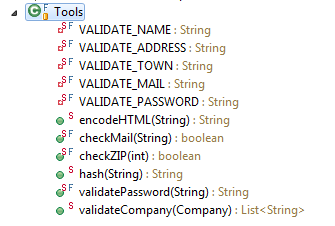
\includegraphics[scale=1]{tools.png}\\
Diese Klasse ist f\"{u}r die Validierung der m\"{o}glichen Eingaben. Wie die Validierung funktioniert wird in einem späteren Kapitel noch genauer erklärt.
\section{Robust Programming}
\subsection{SQL-Injection \& XSS Attacken}
Damit keine Möglichkeit besteht SQL-Injections und Cross-Site Scripting Attacken zu verwenden wurde die Methode $encodeHTML()$ erzeugt. Es wird überprüft, ob der eingegebene Text Zeichen beinhaltet, die zu SQL-Injections oder XSS Attacken führen könnten. Diese Zeichen ``,$<$ und$>$ wurden aber abgefangen und ersetzt mit mit \Bold{''\&\#`` + (int) c + '';``}. Wobei $c$ das momentane Zeichen darstellt. So ist sichergestellt, dass keine SQL-Injections oder XSS Attacken durchgeführt werden können.
\lstinputlisting[caption=HTML Encoding, style=JavaStyle]{encodehtml.java}
\subsection{Validierung}
Wie schon angetönt wurde ist die Klasse Tools für die Validierung der verschiedenen Felder verantwortlich. Es wird nun noch tiefer auf die verschiedenen Methoden eingegangen.
\subsubsection{Variablen}
Die finalen Variablen sind Regexausdrücke. Diese werden benutzt um die Eingaben des Benuters auf Richtigkeit zu überprüfen.
\lstinputlisting[caption=Final Variablen, style=JavaStyle]{finalvariablen.java}
\subsubsection{E-Mail Adresse überprüfen}
Es wird überprüft ob der die E-Mail Adresse die Angegeben wurde auch gültig ist.
\lstinputlisting[caption=E-Mail Adresse überprüfen, style=JavaStyle]{mailcheck.java}
\subsubsection{Postleitzahl überprüfen}
Diese Methode wird im späteren Verlauf noch präziser erklärt.
\subsubsection{Passwort überprüfen}
Ein gültiges Passwort muss mindestens aus 8 und maximal aus 64 Zeichen bestehen. Sonst ist das Passwort ungültig und teilt dies dem Benutzer mit.
\lstinputlisting[caption=Passwort überprüfen, style=JavaStyle]{passwordcheck.java}
\subsubsection{Company überprüfen}
Diese Methode ist für die Verwaltung der Validierung zuständig. \begin{enumerate}
 \item Als erstes wird der Name der Firma überprüft. Dieser darf nicht leer sein, mehr als 20 oder ungültige Zeichen beinhalten. Falls einer dieser 3 Bedingungen verletzt wird, wird dem Benutzer mitgeteilt, welche der Bedingungen verletzt ist.
 \item Als nächstes wird die Adresse überprüft. Die Adresse darf nicht leer sein und keine ungültigen Zeichen beinhalten.
 \item Die Postleitzahl muss im Bereich zwischen $999 < x < 10000$ sein. Zusätzlich muss die Postleitzahl existieren, was wir mit $post.ch$ überprüfen.
 \item Die Stadt muss folgende Bedingungen erfüllen. Das Feld darf nicht leer sein oder ungültige Zeichen benutzen.
 \item Zuletzt wird validiert ob die eingetragene E-Mail Adresse leer ist oder schon einmal benutzt wurde. Zusätzlich wird mit $checkMail()$ überprüft ob diese gültig ist.
\end{enumerate}
\lstinputlisting[caption=Company überprüfen, style=JavaStyle]{companycheck.java}
\subsubsection{Schutz der Model-Klasse vor sch\"{a}dlichem Missbrauch}
Die schwierigkeit einer korrekten Login-implementation liegt darin, den Ablauf so zu gestalten dass nur dieser Ablauf zu einer validen \"{a}nderung f\"{u}hrt. Heisst nur beim vorgesehenen Ablauf k\"{o}nnen nur korrekte Daten geschrieben werden, alles andere darf die Datenbank nicht ver\"{a}ndern. So sind beispielsweise setters auf das Passwort problematisch. Zusammen mit der $.save()$ Methode k\"{o}nnte ein Fehlerhafter oder b\"{o}sartiger Code das Passwort eines beliebigen Users \"{u}berschreiben. Usernamen und ID sind ebenfalls Felder, auf die nur lesend zugegriffen werden soll.

Umsetzung:
Um das Model korrekt umzusetzen wurden zwei Konstruktoren implementiert. Ein Konstruktor nimmt einen Benutzernamen und Passwort entgegen

\subsubsection{Postleitzahl Validierung}
Die Postleitzahl wird mit der Hilfe von post.ch überprüft. Bevor abgefragt wird, ob die Postleitzahl existiert, wird der String in eine Zahl umgewandelt. Dies kann zu einer Exception führen und dann wird zurückgegeben, dass die eingegebene Postleitzahl keine gültige ist.\\
Falls die Postleitzahl nicht existiert wird auf der Seite ``Keine PLZ gefunden'' wissen wir, dass die eingegebene Postleitzahl nicht existiert. Es wird hingegen nicht überprüft ob die eingegebene Postleitzahl mit der Stadt übereinstimmt.
\lstinputlisting[caption=Überprüft Postleitzahl, style=JavaStyle]{checkzip.java}
\subsubsection{SSL}
Damit eine SSL-Verbindung hergestellt werden kann muss man im server.xml etwas aus dem Kommentar herausnehmen.\\
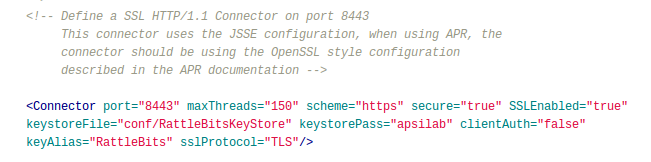
\includegraphics[scale=.5]{ssl.png}\\
Zusätzlich muss man mit dem keystore einen eigenen Schlüssel erstellen.
Damit Login auch eine SSL Verbindung herstellen kann wird im web.xml ein Security Constraint eingebaut.\\
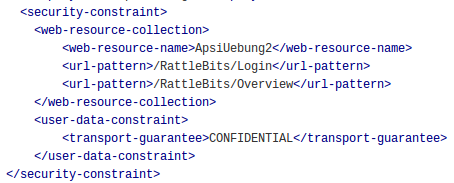
\includegraphics[scale=.5]{web_xml.png}
\section{Weitere M\"{o}gliche Massnahmen}

\subsection{DOS-Attacke}


 \end{document}